\documentclass[oneside,letterpaper]{scrartcl}

% Used Packages
\usepackage[utf8]{inputenc}
\usepackage[english]{babel}
\usepackage{amsmath,amssymb}
\usepackage{graphicx}
\usepackage{hyperref}
\usepackage[]{tocbibind}
\usepackage{wrapfig}
\usepackage{blindtext}

\parindent 0pt

% Commands
\newcommand{\PN}{PyLDTracker}
\def\myscale{0.55}

% Title details
\author{Markus Rose}
\title{\PN\ Quick Guide}
\date{\today}



\begin{document}
\maketitle

\tableofcontents

%==========
\section{About}
\PN\ is a program for localization and detection and tracking of single particles in two-dimensional greyscale TIFF images and videos.

%==========
\section{Installation}

\PN\ is available at \url{https://github.com/MarkusRose/ParticleTracker} under the GPL. It requires a python interpreter, as well as some additional packages listed below. It can be run from the command line, or with a GUI.

\subsection{Getting Python}

\PN\ is written in Python 3.6. The distribution that was used during development and testing is 
Anaconda Python 3 (\url{https://www.anaconda.com/}).


\subsection{Required Packages}

\begin{itemize}
\item numpy
\item scipy
\item pandas
\item matplotlib
\item tkinter
\end{itemize}


\subsection{Running \PN}

\PN is a python 3.6 program. Running it in the interpreter will start the GUI.

\begin{verbatim} python main.py \end{verbatim}

%=================
\section{Using \PN}\parindent 0pt

\subsection{The Graphical User Interface}

\PN comes with a graphical user interface (GUI) written entirely in Tkinter. 

\subsubsection{The Main Window}

\begin{wrapfigure}{r}{0.3\textwidth}
\centering
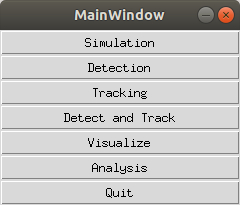
\includegraphics[scale=\myscale]{Figures/MainGUI.jpg}
\caption{Main Menu}
\end{wrapfigure}

The main window shows all available operations than can be performed. Each button opens a new window with the specific option required for the wanted task. The available choices are

\begin{description}
\item[Simulation] A simulation of diffusing particles, which outputs both track files and frame files, as well as a TIFF stack file.
\item[Detection] With a TIFF stack (video) as input file, the fluorescent particles are detected and displayed.
\item[Tracking] Tracking is performed on the file "foundParticles.txt". A TIFF stack can be included, if a visualization is wanted after tracking is complete.
\item[Detect and Track] This option performs the two previous steps with one click. As input file, only a TIFF stack is required.
\item[Visualize] Here either just the TIFF stack, the detections or the full tracks can be displayed. A TIFF stack is required.
\item[Analysis] With a track file as input, various useful analysis tools are located here.
\item[Quit] Exits the program.
\end{description}

\subsubsection{The Simulation Menu}

\subsubsection{The Detection Menu}

\begin{wrapfigure}{r}{0.5\textwidth}
\centering
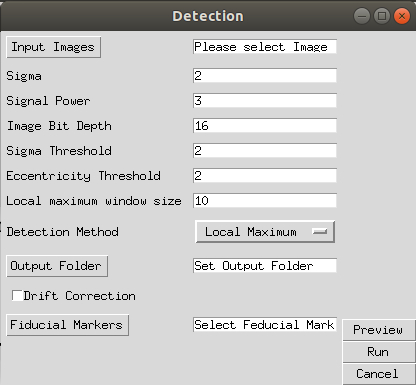
\includegraphics[scale=\myscale]{Figures/DetectionGUI.jpg}
\caption{Detection Menu}
\end{wrapfigure}



\subsubsection{The Tracking Menu}
\begin{wrapfigure}{r}{0.6\textwidth}
\centering
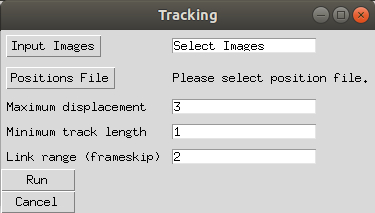
\includegraphics[scale=\myscale]{Figures/TrackingGUI.jpg}
\caption{Tracking Menu}
\end{wrapfigure}


\subsubsection{Detect and Track in one Window}
\begin{wrapfigure}{r}{0.6\textwidth}
\centering
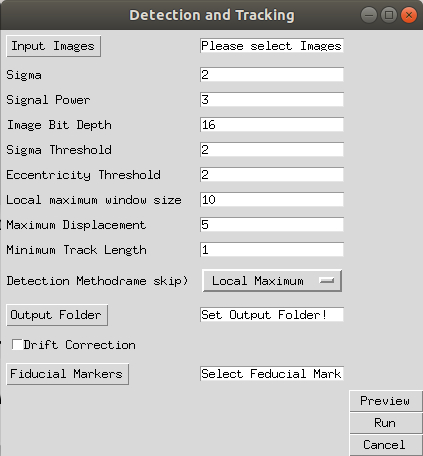
\includegraphics[scale=\myscale]{Figures/DetandTrackGUI.jpg}
\caption{Detect and Track Menu}
\end{wrapfigure}


\subsubsection{Visualization of Images, Detections and Tracks}
\begin{wrapfigure}{r}{0.6\textwidth}
\centering
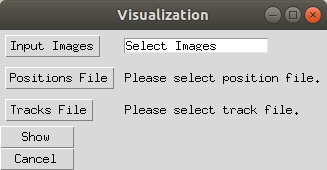
\includegraphics[scale=\myscale]{Figures/VisualizationGUI.jpg}
\caption{Visualization Menu}
\end{wrapfigure}


\subsubsection{Simulation Window}
\begin{wrapfigure}{r}{0.6\textwidth}
\centering
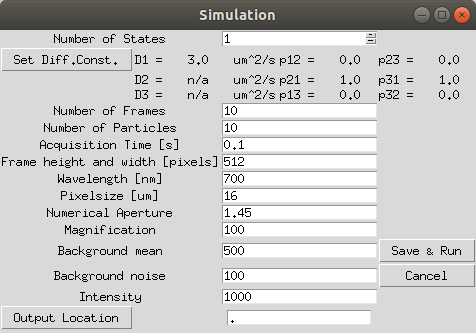
\includegraphics[scale=\myscale]{Figures/SimulationGUI.jpg}
\caption{Simulation Menu}
\end{wrapfigure}


\subsubsection{Analysis Tools for obtained Tracks}
\begin{wrapfigure}{r}{0.6\textwidth}
\centering
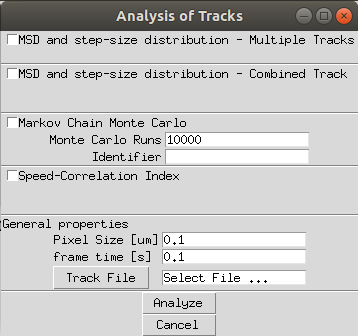
\includegraphics[scale=\myscale]{Figures/AnalysisGUI.jpg}
\caption{Analysis Menu}
\end{wrapfigure}


\subsection{Working from Command Line}

%=================
\section{Program Output}

\bibliographystyle{ieeetr}
\bibliography{biblio}

\end{document}
